%----------------------------------------------------------------------------
\chapter{Design and implementation}
\label{chap:designimplementation}
%----------------------------------------------------------------------------

Let's recap the task flow of the task I described in the Introduction: After
configuring the simulator with the designed camera setting I render multiple
traffic scenarios in different maps provided by CARLA while extracting all
necessary information into a log file to later compare the detection log with


\begin{figure}[!ht]
    \centering
    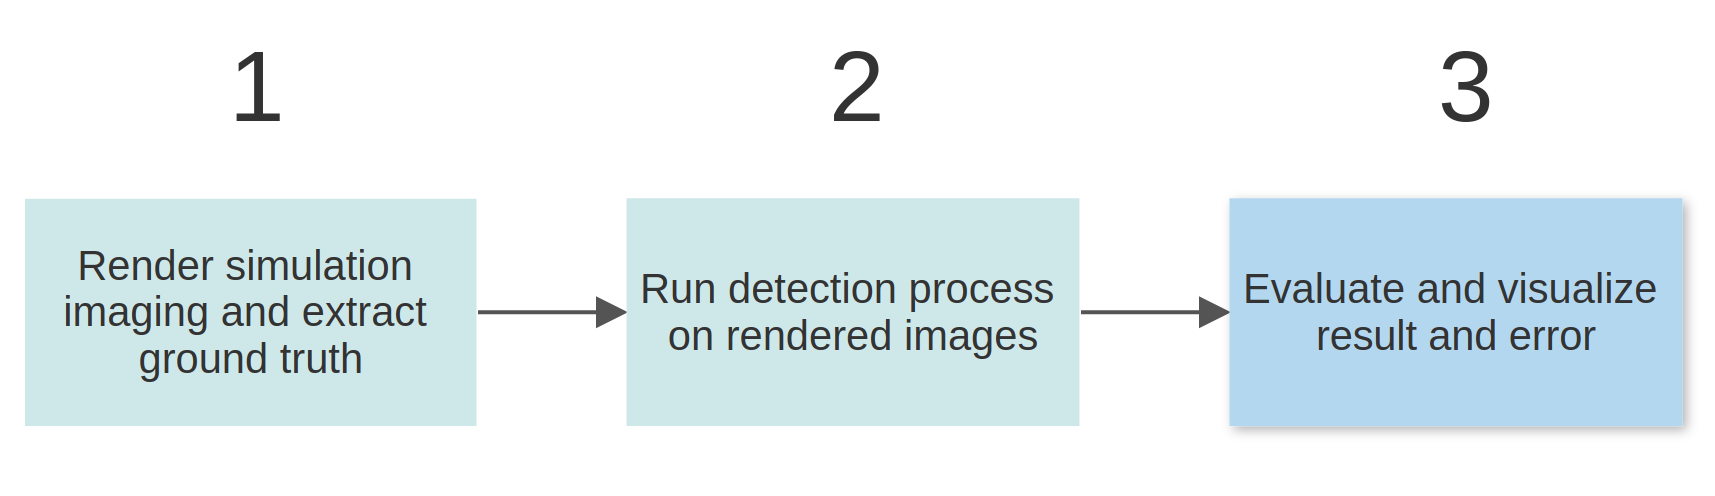
\includegraphics[width=150mm, keepaspectratio]{figures/flowchart.png}
    \caption{Task flow}
    \label{fig:flow2}
\end{figure}


\section{Tools used}

Soon it became obvious that Linux operating system is the right tool to use
for development. I have been using Ubuntu before this project as well so I was
already familiar with everything. The main IDE I used throughout the project is
Visual Studio Code, which thanks to it's openness and community has many useful
extensions that helped me develop in fact every part of the thesis: Python,
Nodejs and Javascript for the webvisualizer and finally LaTeX and ofcourse git
support.

I also used Conda which is I think an essential tool when you want to develop ML
and AI projects with Python. Conda makes it easy to create and use separate
Python environments. This is important because different implementations of
algorithms require different versions of the same packages thus it keeps a clean
separation. The drawback is that consecuently it requires an excessive ammount
of hard-drive space.

Upon developing the algorithm and experimenting with it I used Jupyter Notebook
which is a Python runtime on top of the bare one and a web-based IDE at the same
time. With Jupyter Notebook it is easy to change and re run the code thanks
to it's "kernel" system, which keeps the value of variable and imported packages
between executions.

For the GPU-intensive tasks such as simulation and convnet calculations in the
detector I was provided with a remote Titan X GPU\footnote{ Titan X GPU
    \url{https://www.nvidia.com/en-us/geforce/products/10series/titan-x-pascal/}} by
my university.

\section{Choosing the sensor suite}

Mounting cameras around the vehicle to have an all around vision is an essential
design strategy, as we have seen in the work of other companies in
\autoref{chap:relatedwork}. However we will need to determine depth as well. I
decided to use only cameras in a stereoscopic structure to create 5 stereo sides
around the vehicle. The following image shows the design setting with field of
views visualized in \autoref{fig:3dmodel3}.

\begin{figure}[!ht]
    \centering
    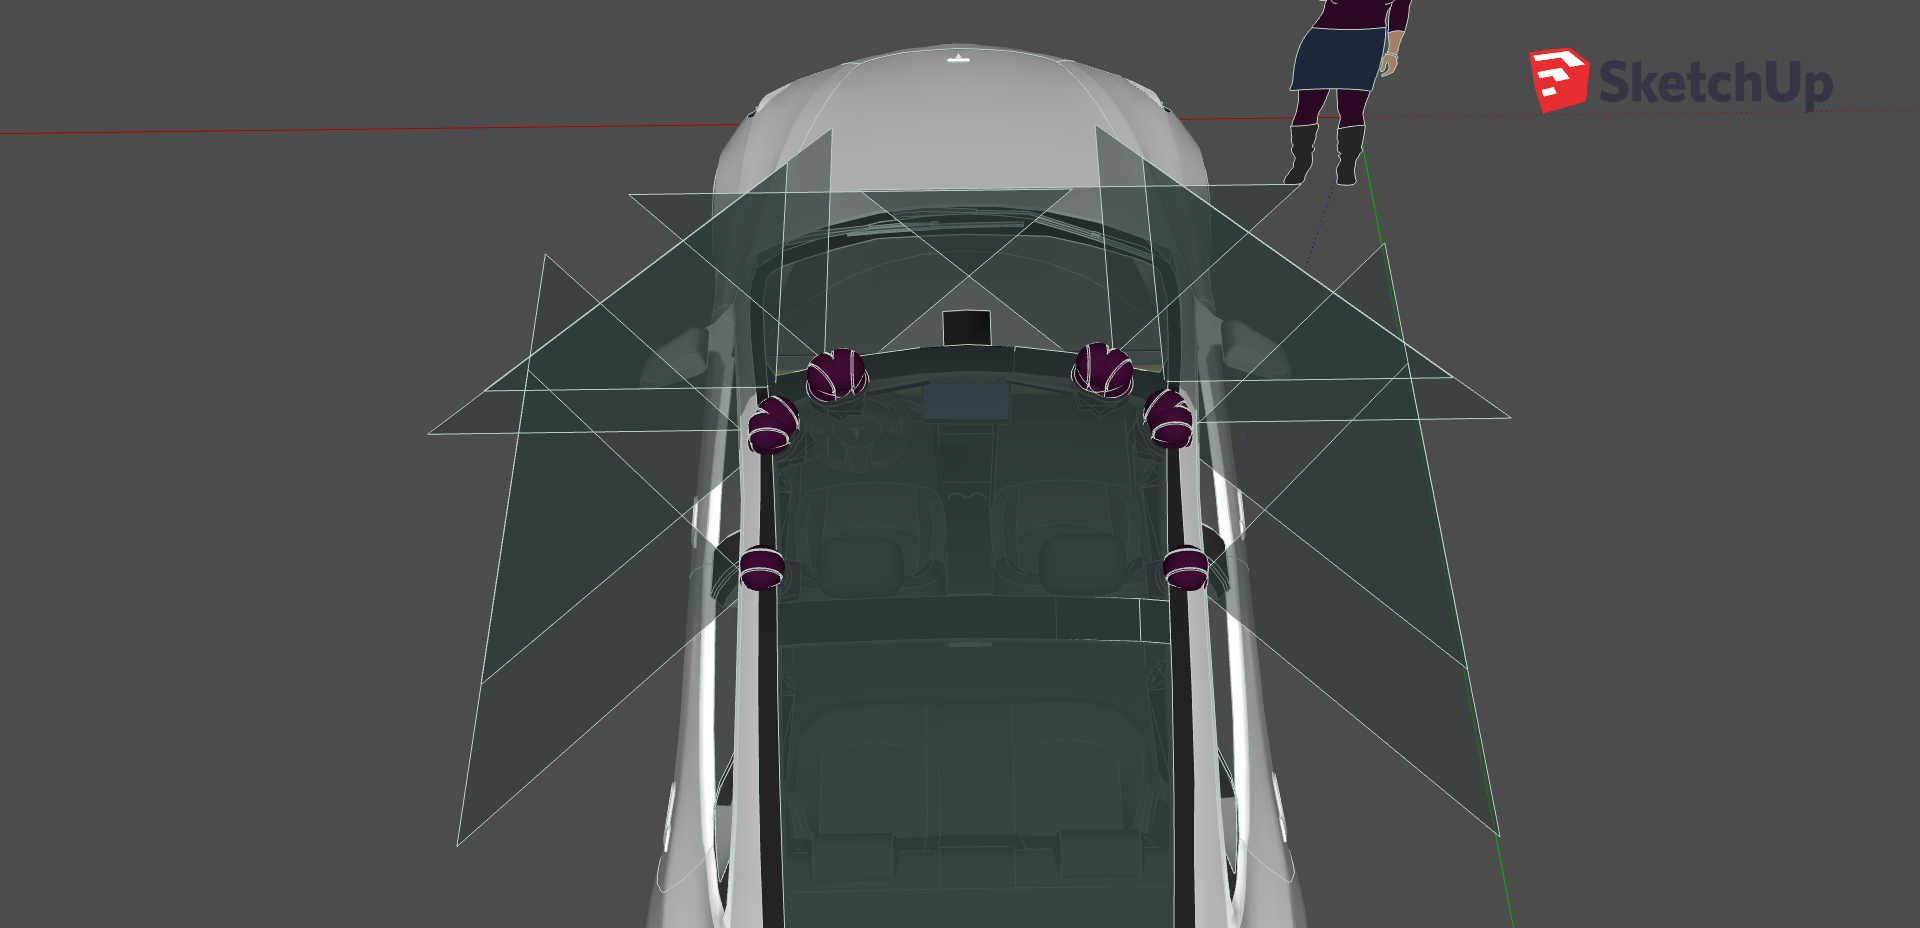
\includegraphics[width=150mm, keepaspectratio]{figures/3dmodel3.png}
    \caption{The stereo camera setting I used on top of the virtual Tesla Model 3}
    \label{fig:3dmodel3}
\end{figure}

In details: 
\begin{itemize}
    \item Front stereo: two cameras looking straight to the front 0.8 meters
          apart
    \item Right corner and left corner stereo cameras: the cameras are on the
          diagonal corners of a 20 cm wide 20cm tall triangle creating two 45\degree
          angled stero vision.
    \item Right and left side stereos are turned 90\degree to the sides and they are apart 0.5 meter.
\end{itemize}
The cameras are 1.5 meters above the ground and they are mounted relative to the
bottom center-point of the vehicle.

The advantage of puting stereo cameras apart to a relatively large distance is
that it increases the accuracy of the stereo block matching algorithm to a
further distances. The drawback however is that a smaller portion of the right
and left side images are going to intersect hence creating a smaller field of
view. However due to the corner stereo cameras this is not a problem for us.

\section{Configuring the simulation}

Carla simulator can be ran in two time-step settings: variable and synchronous.
In real-world perception it is a complex task by itself to synchronize multiple
cameras with each other so that when the algorithm calculates information based
on data from multiple sensors they all correspond to the same moment in time
with an error boundary. In a simulation however we can have the freedom to
synchronize the simulation timesteps themselves and collect all imaging data
between each timestep. Setting Carla to synchronous timestep ensures that all
images in a certain frame are collected and respond to the same moment. 

I used 30FPS timestep setting so that physics calculations are still realistic
but the performance is not too bad. We also have to account for the size of the
generated images: it was good to half the size of the image datasets from a
60FPS setting. Increasing the traffic participants also degrades the
performance. I usually used 200 vehicles and 100 pedestrians for each map, that
resulted in realistic traffic scenarios. 

I recorded different scenarios of approximately 1 minute, which means 1800
frames on 30FPS. On the Titan X machine it it took 15 minutes to render 1
simulation minute, i.e. it ran the simulation with 2FPS. Note, this is different
from the simulation time-step which we fixed to 30FPS.  Since I collect 10 images
in each frame it results in a dataset of 18000 images.

The camera setting I used is an undistorted camera that takes $1280\times720$
resolution images, i.e. HD 720p images, compressed with JPEG to yield a
reasonable size. This way one image is on average 215 kilobytes instead of 1MB
which is a good compression rate and this was the limit where I did not see
any difference in detection accuracy.

In a real-world systems images go straight to the GPU and CPU unit and they get
downscaled to the choosen size before feeding into the algorithm. I had to
resort to compression because of the research nature of the project: I reran
and tested the accuracy of the detector many times on the same dataset.

Using an undistorted camera matrix only means that we need to use one less back
transformation matrix in the detection calculations. In real-world the intrinsic
camera matrix is calculated and corrected for cameras that are mounted on cars
and it is part of the calculation.

Besides imaging we have the ground truth log data. During the simulation,
besides rendering images I coded a logger that logs the necessary information of
the state of the simulator for each frame. This information is built up in a
json-like dictionary, and at the end of the simulation it is saved to one file,
that I call the framelist.

\section{Extracted data}

Naming the images in an organized way is important to make it easy to read the
images in a structured way upon detection. Each image starts with the number of
the frame it was taken in. Starting the simulator server Carla increases a
frame counter starting with 1. To know which image corresponds to which camera,
the framenumbers are postfixed with a label. \autoref{fig:labeling} shows the
postfixes for each image.

\begin{figure}[!ht]
    \centering
    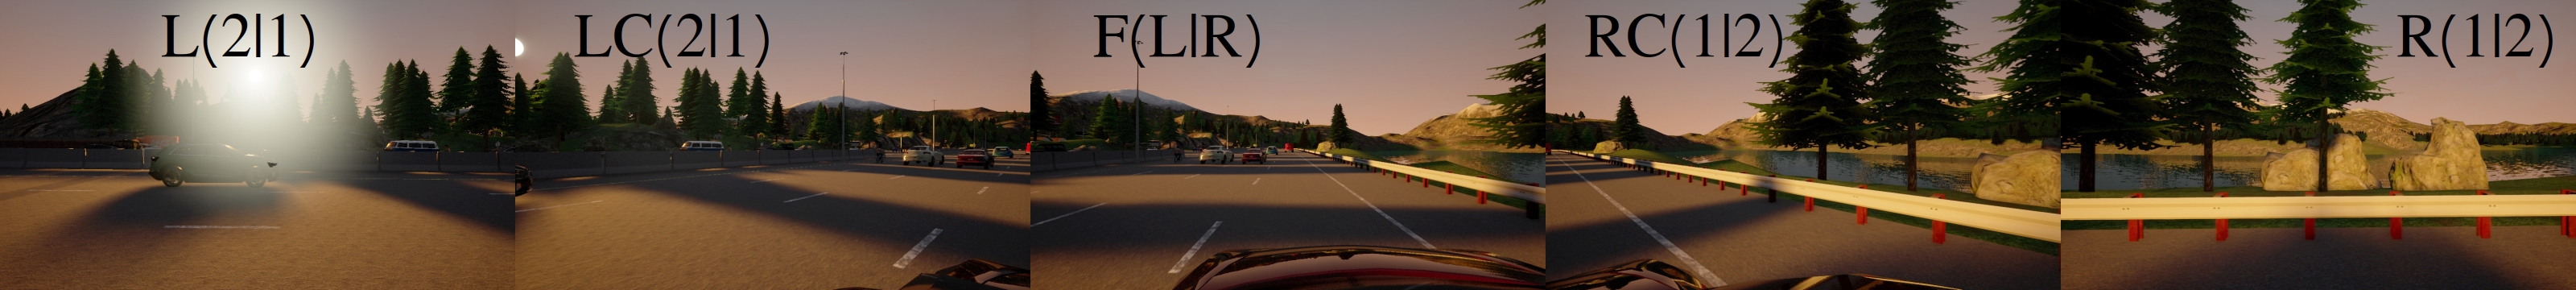
\includegraphics[width=150mm, keepaspectratio]{figures/labeling.jpg}
    \caption{L2/1, R1/2: Right side/Left side first and second cameras, LC(2/1), RC(1/2): Right corner, left corner cameras, FL FR: Front left, front right cameras}
    \label{fig:labeling}
\end{figure}

In each frame I log information about the current state of the simulation. For
the purpouses of the final detector the following information gets logged in each frame:
\begin{itemize}
    \item Frame's number: the value of the frame counter at each frame
    \item For all walker and vehicle actors in a 100 meter radius from the ego car:
          \begin{itemize}
              \item Id: corresponds to the actor's unique id among other actors.
              \item Relative position: X, Y, Z coordinate of the actor in the CARLA
                    coordinate system (see \autoref{fig:carlacoords})
              \item Distance: Euclidean distance from the ego car
          \end{itemize}
    \item Waypoints: these are center and left-right points of the lane the egocar is currently in up
          to 30 points forward. These were meant to be the ground-truth data for
          lane-detection
\end{itemize}

This information is then exported into a JSON file with the following format:
\begin{lstlisting}[language=]
frameList: [
    {
        frame: Number,
        actors: [
            {
                type: car|pedestrian,
                id: Number,
                relative_position: {
                    x: Number,
                    y: Number,
                    z: Number,
                }
            },
        ],
    },
]
\end{lstlisting}

For a one-minute simulation the ground-truth json file is approximately 20
megabytes. It isn't optimal to save information like this for longer
simulations. In those cases it is recommended to use a binary format. Carla
provides a way to save binary information of the recording but unfortunately
there were issues with recording that way, so I ended up with this custom log
format. However it ended up being beneficial, because the webvisualizer
simply loads the json files (detection and ground truth) into two JavaScript
objects.

\section{Detector}

The algorithm plan is the following: for each stereo pair of images calculate
the disparity map with a stereo block matching algorithm. Then detetect objects
and their segmentation mask (instance segmentation) with a state-of-the-art
convnet and then extract the disparity data using the segmentaiton mask. Then
use the extracted disparity data to estimate the depth of the detected object and
then reproject to Carla-world coordinates to match the logfile coordinate
system.

\subsection{Detectron2}
Detectron2's~\cite{wu2019detectron2} Mask R-CNN model provides both object
detection and instance segmentation so I decided to use it. Detectron is built
with PyTorch, Facebook's own GPU-aided ML library.

% There are multiple models provided by D

The algorithm runs the detecton prediction only on the left image of each side,
because later on we will need the segmentation mask of the left image to extract
the depth data from the disparity map generated by the stereo block matching
algorithm. 

Before prediction if our ego car falls into the image it is filled with zeros,
i.e. it is occluded ith black color. It is better to use black since it is all
zeros, and therefore convnet is not going to be sensitive for those parts of the
image.

A visualization of the detection results can be seen on \autoref{fig:detection}

\begin{figure}[!ht]
    \centering
    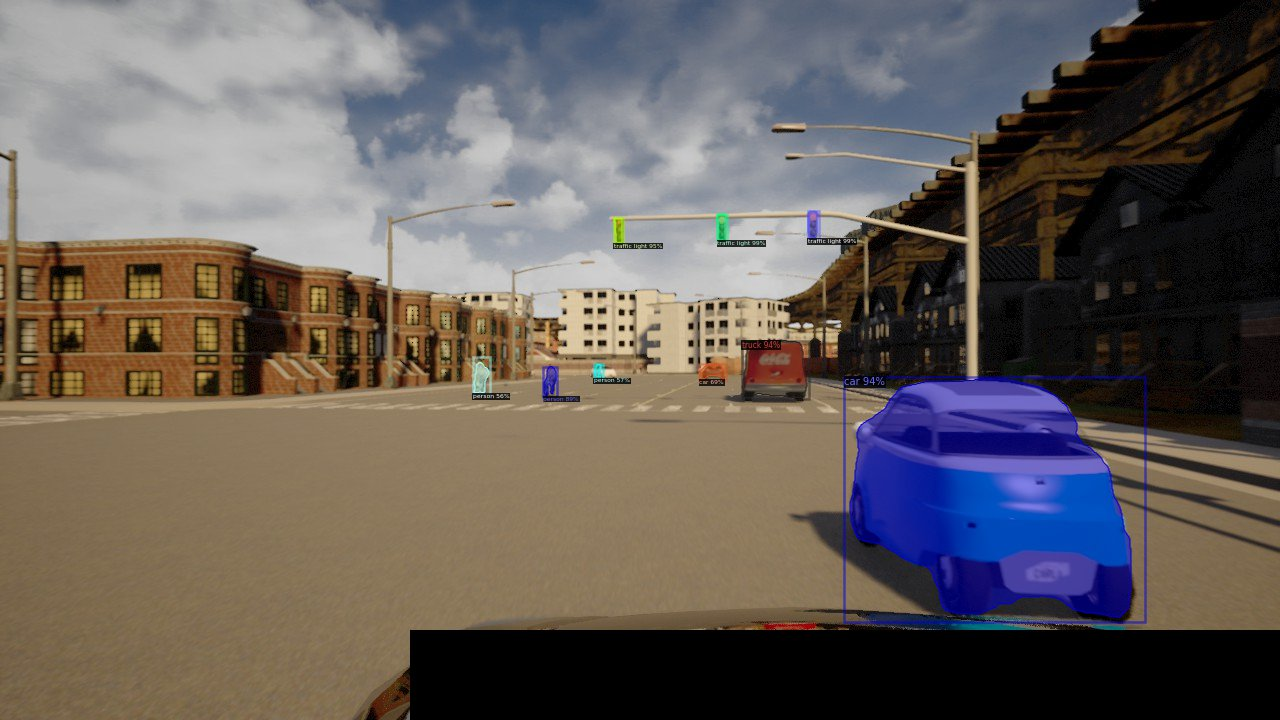
\includegraphics[width=150mm, keepaspectratio]{figures/335DET.jpg}
    \caption{A visualization of the Detectron2 detections and instance segmentation on an ego-occluded image}
    \label{fig:detection}
\end{figure}

\subsection{Depth estimation}
To perform depth estimation I found to easiest way is to use OpenCV a widely
used library in computer vision that includes the stereo processing tools I
needed.
\subsubsection{OpenCV}
OpenCV is a library of programming functions mainly aimed at real-time computer
vision originally developed by Intel. The library is cross-platform and free for
use. It provides traditional Computer Vision tools such as the stereo
correspondence algorithm using block matching~\cite{5489515} and an advanced
version of it the Semi-Global Block Matching method (SGBM)~\cite{4359315} that I used
for the stereo disparity map calculation.
\subsubsection{Stereo Block Matching Algorithm}
The Stereo Block Matching Algorithm works by comparing the neighborhood of a
pixel to each neighborhood of the row of the other image - the measure of
similarity can be different, but usually the mean squared error is used. Usually
before using the stereo block matchin algorithm a camera calibration is
required. This happens with the chessboard calibration method
\footnote{Chessboard calibration in OpenCV \url{https://docs.opencv.org/master/dc/dbb/tutorial_py_calibration.html}}
 where a flat checkerboard is displayed in front of the two stereo cameras. The
 calibration algorithm then calculates the distortion for each camera and
 rotation difference between the two cameras to calculate the intrinsic matrix.

 In our case since we record images in a super ideal way: no distortion and
 perfectly parallel cameras we don't need any calibration and application of
 inverse intrinsic matrix before using the SGBM algorithm.

\begin{figure}[!ht]
    \centering
    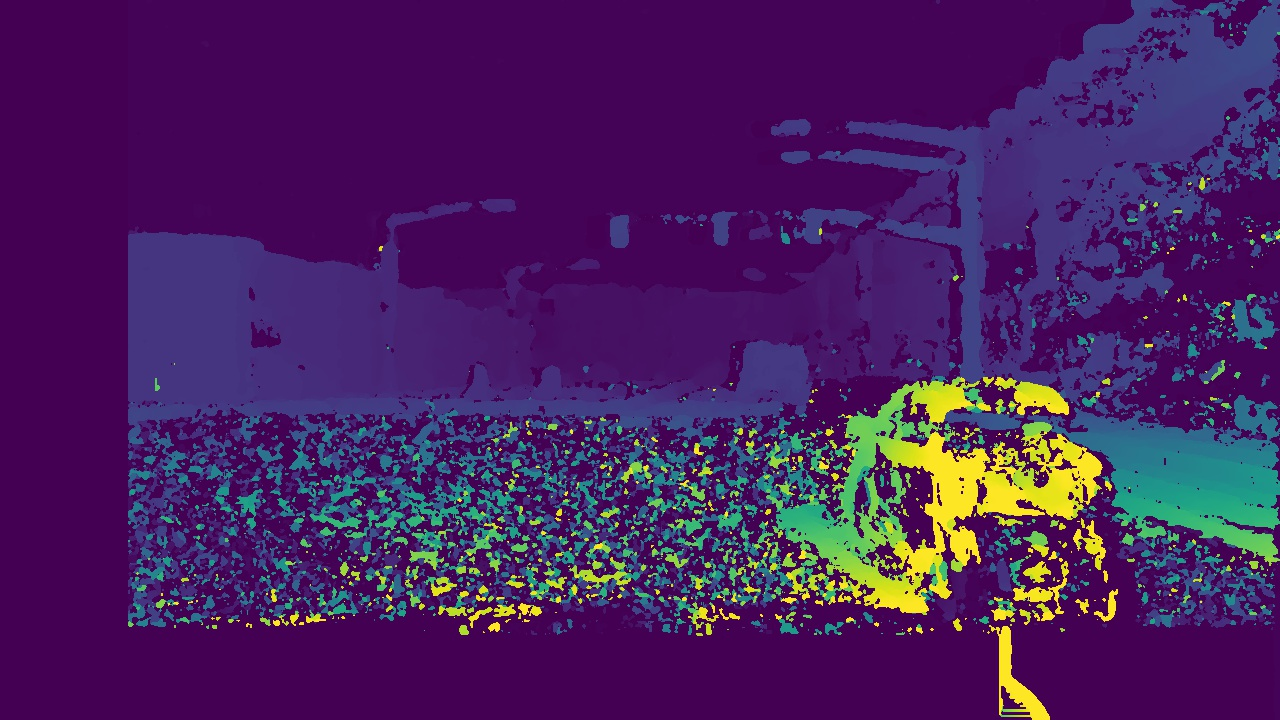
\includegraphics[width=150mm, keepaspectratio]{figures/335DP.jpg}
    \caption{A visualized disparity map result after using OpenCV's StereoSGBM algorithm on the front stereo side}
    \label{fig:disparitymap}
\end{figure}

The StereoBM algorithm considers the left image as the primary, so it will
return a disparitymap that corresponds to the pixels of the left image.

\subsubsection{Triangulation}

Triangulation is a simple method of deriving the depth coordinate when we have
two parallel cameras. \autoref{fig:triangulation} shows the camera setting of
an ideal stereo setting. Recall, that each stereo side in our setting is like
this.

\begin{figure}[!ht]
    \centering
    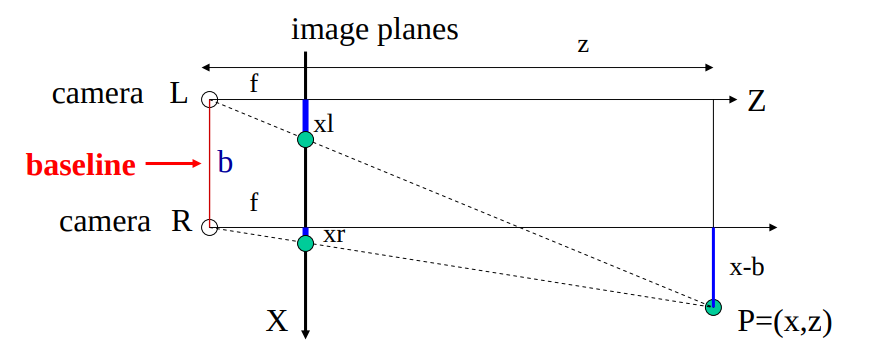
\includegraphics[width=150mm, keepaspectratio]{figures/triangulation.png}
    \caption{An ideal parallel stereo camera model.}
    \label{fig:triangulation}
\end{figure}

If there is a point P in the real world in the field of view of the stereo
camerase, the point will be projected onto different points of both camera's
image plane. If the cameras are set in an ideal parallel stereoscopic setting
then we can easily calculate the depth of the point. The pixel difference
between between pixels correspoonding to the same block can be calculated with
xr-xl. The OpenCV Stereo BM algorithm provides this value for each matched
pixel. From now on all we have to do is use triangulation to calculate the depth
of each pixel. The f corresponds to the focus length and Z corresponds to the
real depth of the point.

The following equations hold true for the figure above from similar triangles.
\begin{align}
    \begin{split}
        \frac{z}{f} = \frac{x}{xl} =  \frac{x-b}{xr} \\
        \frac{z}{f} = \frac{y}{yl} =  \frac{y-b}{yr}
    \end{split}
\end{align}

From this the triangulation is as follows:

\begin{align}
    \begin{split}
        \text{Depth}\;\; Z = \frac{f \cdot b}{xl - xr} =  \frac{f \cdot b}{disparity} \\
        X = \frac{xl \cdot z}{f} \\
        Y = \frac{yl \cdot z}{f}
    \end{split}
    \label{eq:depthcalc}
\end{align}

Where xl and yl refers to to distance from the center of the image to the center
points of the detection boundingbox (in the left image). 

\subsubsection{Depth calculation}
Now we know the way to calculate the depth knowing the disparity. The result of
the SGBM, seen on \autoref{fig:disparitymap}, is a 2D array containg valid and
invalid data values. In order to determine the right disparity value
for a detection it is not enough to simple take the values under the mask. The
disparities under a mask contain values for the same object's closest point and
farthest point from the camera. Taking into account the simplifications we
established in the previous chapter there are two solutions to find the distance
of the object: 1.) take the average of the valid disparities under a mask 2.)
take the mode of the disparities. By intuition we would choose taking the
average, however that is going to result in high error and high variance. The
reason is, that the segmentation itself is going to mask values that might not
correspond to the object's disparities. Even a few values that are far from the
average the object's disparities can change the average of the masked
disparities drastically. Using the mode the algorithm yielded much more stable
results, that way it simply is ignores the small inaccuracies of the masking and
disparity error and takes the most dominant disparity value. The visualization
of masking can be seen on \autoref{fig:merged}.



\begin{figure}[!ht]
    \centering
    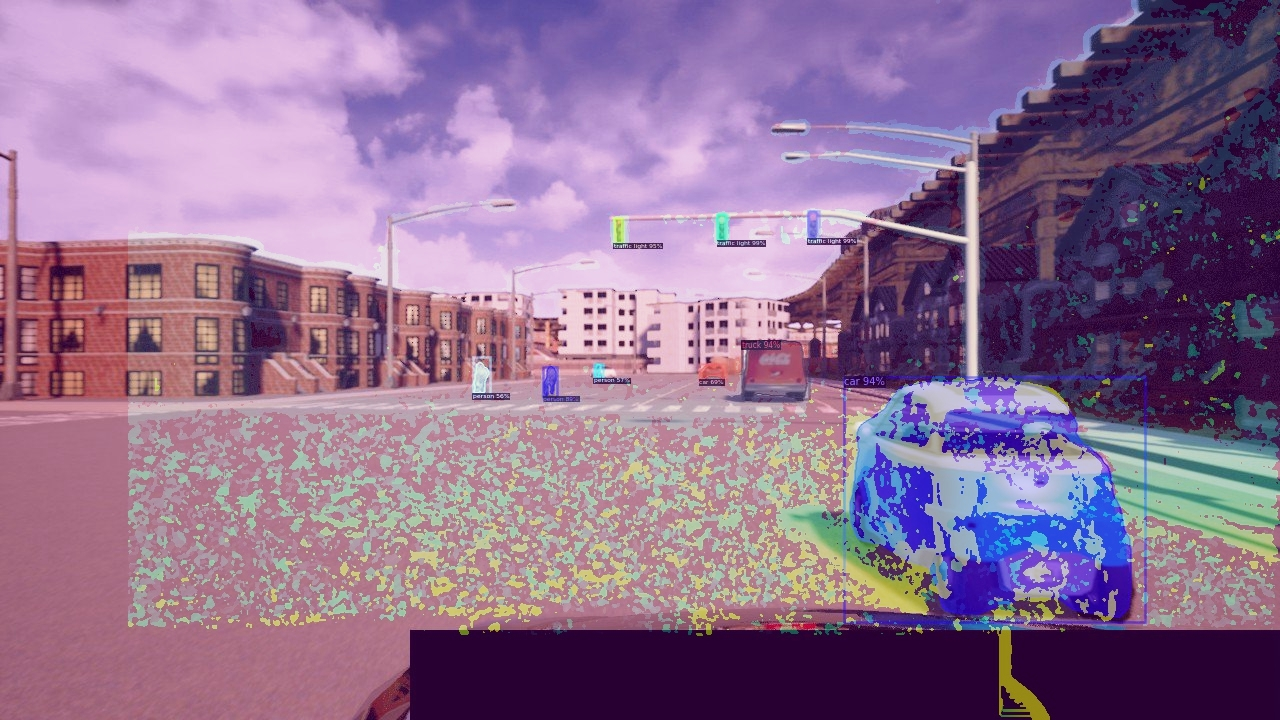
\includegraphics[width=150mm, keepaspectratio]{figures/335merged.jpg}
    \caption{Masking the instance segmentation with the disparitymap filters the necessary values for estimating the vehcile's depth}
    \label{fig:merged}
\end{figure}



\subsection{Back projection}
Each stereo side has a transformation matrix initialized before running the
algorithm. Each matrix is an affine 4x4 transformation matrix, that does the
following in this order: 
\begin{enumerate}
    \item It swapes the axes from the image coordinate system to Carla's coordinate system z->x, x->y, y->z
    \item It rotates the points with the same rotation as the camera
    \item It translates the camera with the same translation for the camerase relative to the vehcile's bottom center point.
  \end{enumerate}

The resulting x, y, z coordinates are the final detection coordinates that go into the detection log.

\subsection{Final pseudo-code}
The final algorithm pseudo-code:
\begin{lstlisting}[language=]
for each frame:
    for each stereo side:
        1. read left and right image
        2. occlude ego from image
        3. compute disparity map using stereo bm.
        4. predict detections and instance segmentation
        for each detection:
            mask disparity map with detection segmentation
            calculate mode of the masked disparity
            apply triangulation and inverse projection
            add actor to frame
    add frame to framelist
save detection list
\end{lstlisting}

\section{Web visualizer}
As I mentioned before in order to compare the detection result and the ground
truth log of each rendering scenario it would be useful to have a visusalization
of the detection replayed. This is similar to the information shown on a monitor
of a self-driving car.

Since I already had experience in Javascript and in ReactJs \footnote{ReactJs
    \url{https://reactjs.org/}} - an easy-to-use web application framework
developed by Facebook - I decided to look for options in 3D visualization. I
found WebViz\footnote{WorldView WebViz \url{https://webviz.io/worldview/}}, a
React library specifically made for 3D visualization of traffic scenarios. It
has a compelling declarative API.

There are two main views in the end product webvisualizer: The video montage and
the 3D visualization (\autoref{fig:webviz2})

The main feature of the webvisualizer is to replay each simulation and see the
original, detection and depthmap videos in synchronization with the 3D
visualizer that displays both the detection log and the ground truth log for
each frame. The webapp is equipped with control buttons that help the control of
the playback. 

\begin{figure}[!ht]
    \centering
    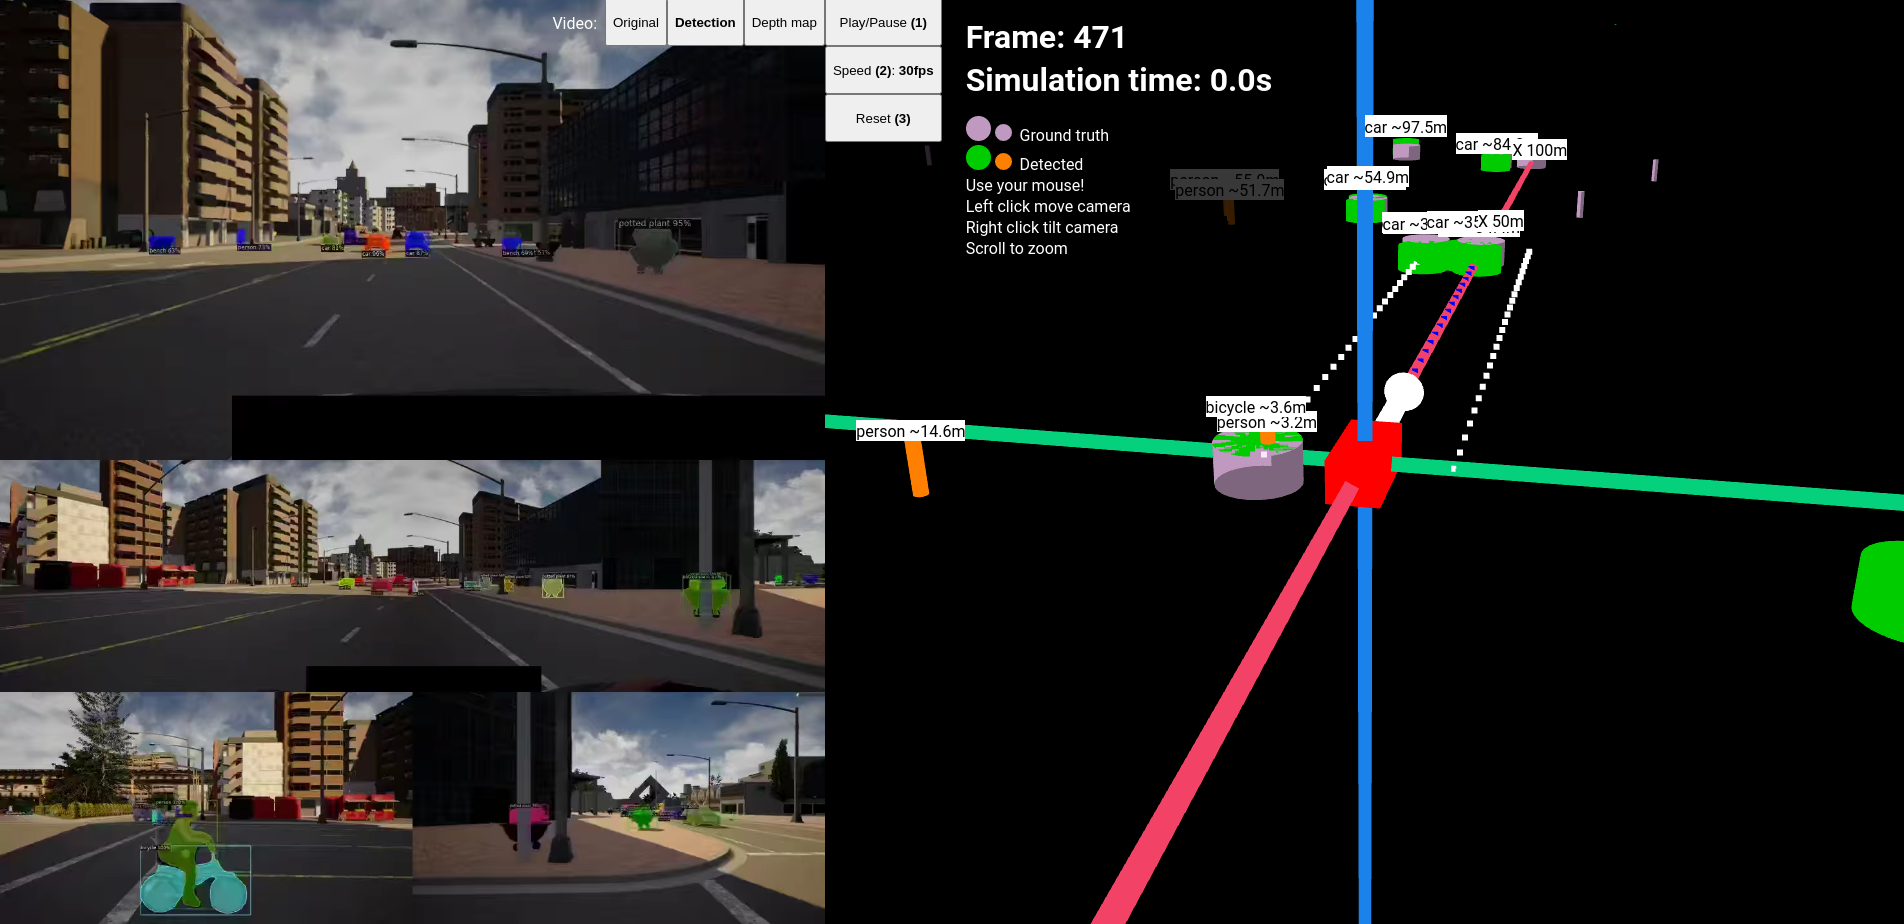
\includegraphics[width=150mm, keepaspectratio]{figures/webviz3.png}
    \caption{Screenshot of the webvisualizer}
    \label{fig:webviz2}
\end{figure}

\begin{figure}[!ht]
    \centering
    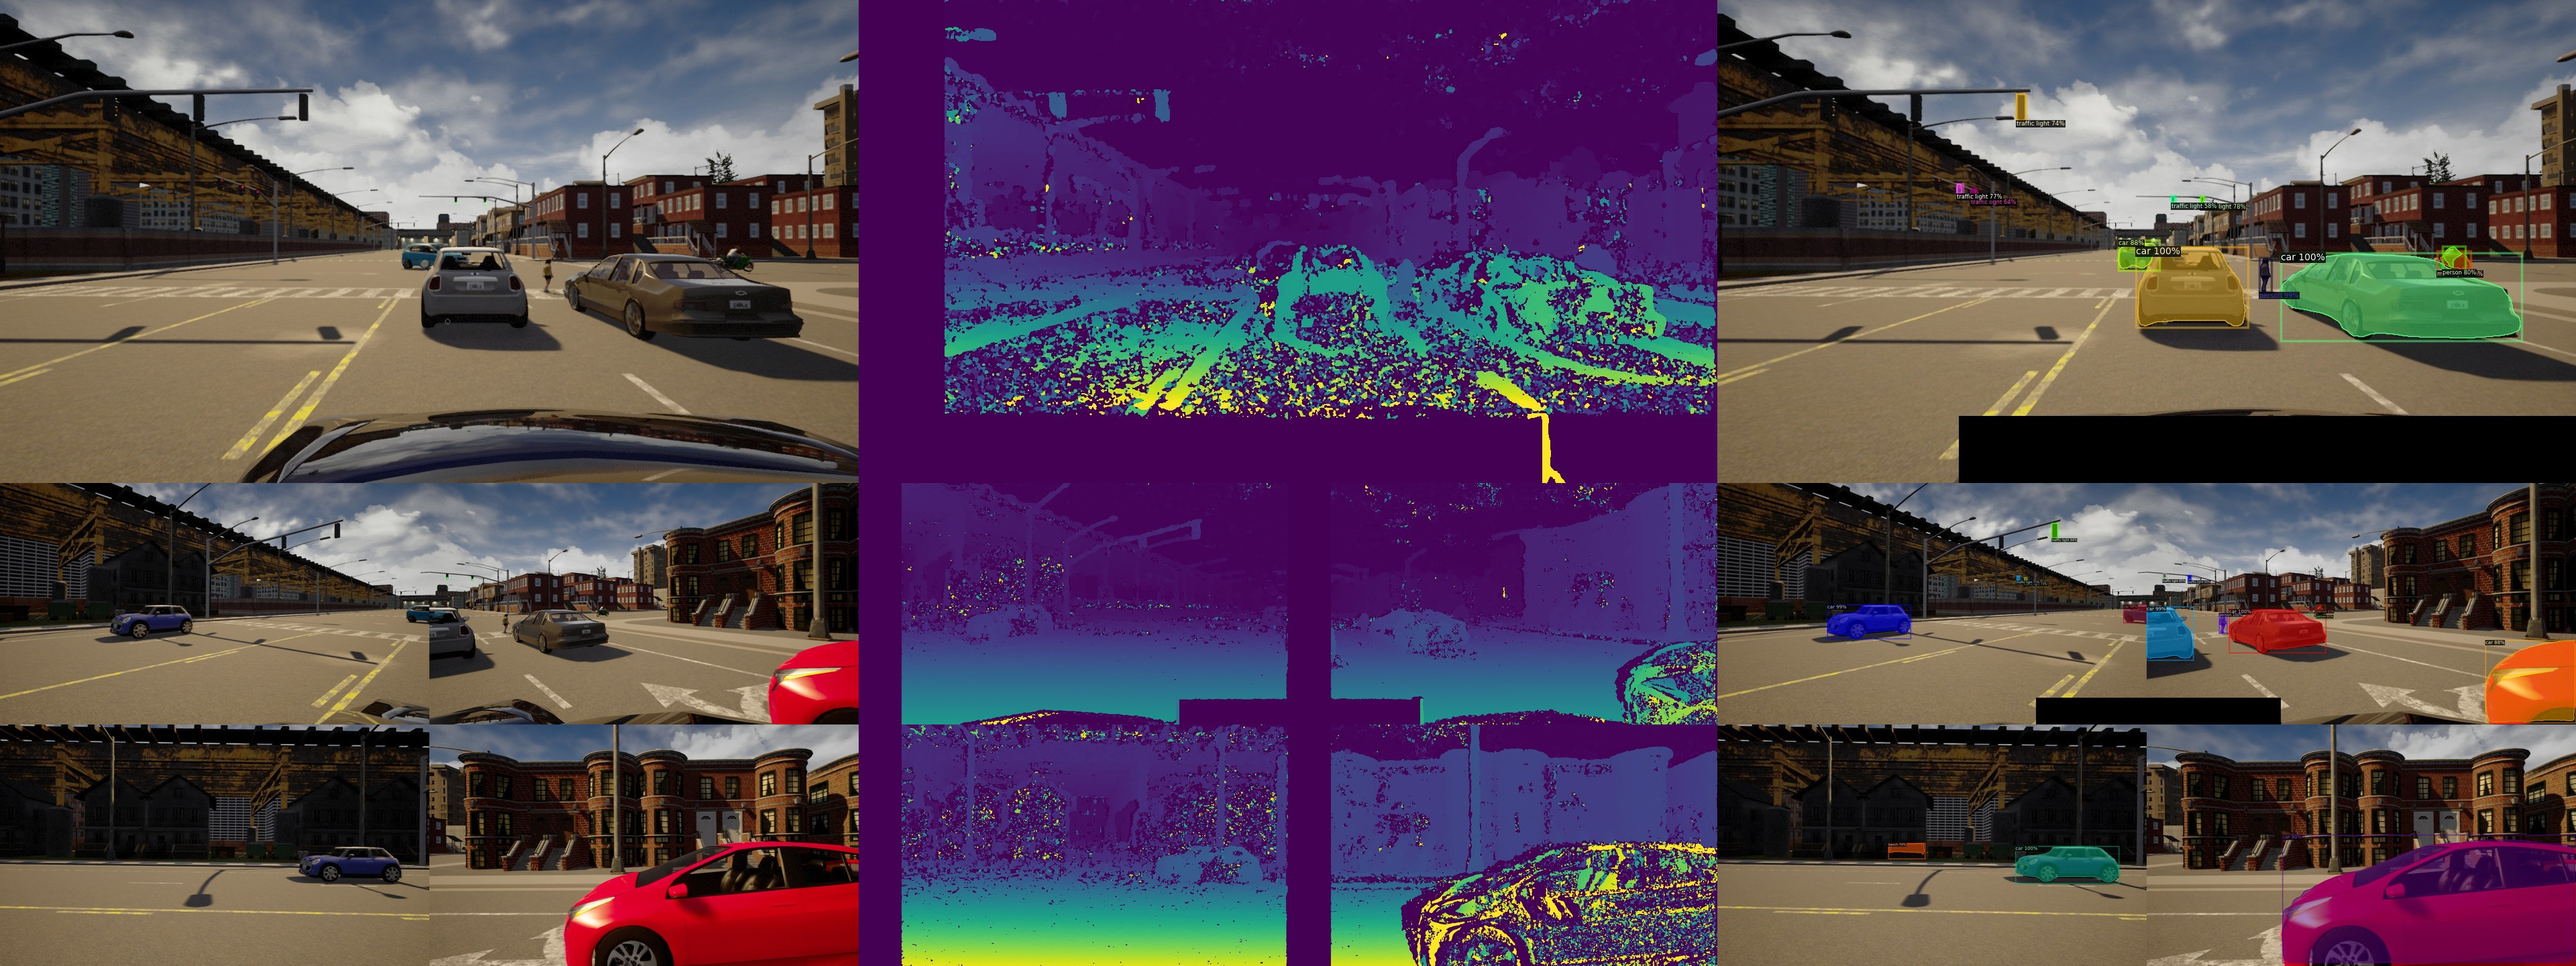
\includegraphics[width=150mm, keepaspectratio]{figures/detmontage.jpg}
    \caption{The montage videos in the webvisalization: original, depthmap, detections}
    \label{fig:detmontage}
\end{figure}


\section{Additonal scripts}

In order to simplify some tasks that included multiple repetitive commands I had
to create some scripts that let me invoke them in one command. One script was to
start the simulator, the ego controller and spawn actors in a choosen map all in
one script. Another useful script was to create a montage of all frames and
immediately create a video and compress it multiple times.
